\documentclass[12pt]{article}
\usepackage[english]{babel}
\usepackage{enumerate, setspace, float, stackengine}
\usepackage[hidelinks]{hyperref}
\usepackage[margin=1.5cm]{geometry}
\usepackage{caption, subcaption}
\usepackage{amsmath, amsfonts, amssymb}
\usepackage{fontspec}   %加這個就可以設定字體
\usepackage{xeCJK}       %讓中英文字體分開設置
\setCJKmainfont{標楷體} %設定中文為系統上的字型,而英文不去更動,使用原TeX字型

\title{\textbf{Theory of Computer Games}\\ Final Project - Dark Chess}

\author{R04922058 鄭以琳}
\date{\large \today}


\begin{document}
\maketitle

\section{Introduction}
Based on the given template codes, I implemented NegaScout searching procedure with a more advanced evaluating function. Transposition table is used to improve the efficiency. I also put effort in writing knowledge-based rules such as decision between moving and turning over a piece.

\section{Implementation}
\subsection{Searching Algorithm - NegaScout}
	I implemented NegaScout algorithm in this project. Before searching with $[\alpha, \beta]$ window, perform a null window search to get a better chance of pruning further branches.
	\paragraph{Quiescent search}
	When encountered a terminal node, instead of directly returning the evaluated value of the current board, a quiescent search is invoked to avoid the horizontal effect. In quiescent search, only eating moves are considered. The evaluating function is called when there exists no capturing moves, or when capturing pieces is not the best choice.
	\paragraph{Iterative Deepening}
	Since the time for thinking is limited, I used iterative deepening so that when it's going to run out of time, the program stops searching deeper and returns the current best move. Iterative deepening can also be used to obtain a better move ordering. According to results from the previous iteration, NegaScount can search children with high scores first.
	\paragraph{Null Moves}
	In some situations, a player may decide to turn a piece instead of moving a piece. Therefore, the evaluation may be inaccurate if searching algorithm only considers moving face-up pieces. However, enumerating all possibilities of turning pieces is inefficient. Thus, I allow players to do null moves when there exists face-down pieces on the board to capture the idea of turning pieces.
	
		
\subsection{Decision between Moving and Turning a Piece}
 	For every face-down piece $p$, and every possible kind of piece $k$ that $p$ may be, the program calculates the score of board after turning $p$ to become $k$ and simulated 4 plys. Take Figure \ref{fig:turn} for example, there are 3 face-down pieces \textit{a2}, \textit{b5} and \textit{d2}. There are also three kinds of pieces these $p$ may be, which are red Guard, red Cannon and black Mister. Thus each $p$ will have three scores, indicating the score of board after 4 plys when $p$ is red Guard, red Cannon and black Mister individually. Compare these scores with the best score of moving a face-up piece. If turning a piece has a good chance to achieve a better score (probability of "turning score greater than moving score" is greater than 0.5), the program will turn the piece with the highest sum of scores; otherwise, the program will move a face-up piece.
 	
 	
 	\begin{figure}[H]
	\centering
	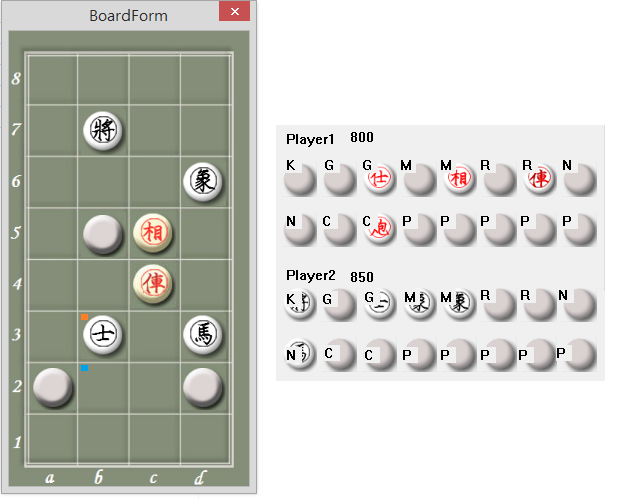
\includegraphics[width=0.6\textwidth]{fig_turn}
	\caption[Caption for the list of figures]{}
	\label{fig:turn}
	\end{figure}

\subsection{Evaluating Function}
	Evaluating function in my program is consists of two parts.
	\paragraph{Material Value}
		The values of pieces are set to:
			\begin{table}[H]
			\centering
			\label{my-label}
			\begin{tabular}{ccccccc}
			King  & Guard & Minister & Rook & Horse & Cannon & Pawn \\
			12863 & 6431  & 3215     & 1607 & 803   & 805    & 200 
			\end{tabular}
			\end{table}
			
	When a kind of my piece can't capture any piece on the board, I set the material value of that kind of piece to 0. In this way, I can sacrifice those useless pieces in the end game if needed.
	\paragraph{Position Value}
		Generally, the side with the greater mobility, other things equal, has a better chance to win. My program calculates the absolute positional information, i.e. how many choices of moves a piece have.

\subsection{Transposition Table}
	Transposition table saves the evaluation values for boards calculated before. An entry of the table includes the searching depth, the player makes the last move, the evaluated score of the board and the type of value(lower bound or exact). I implemented Zobrist Hashing with 32-bit keys and $2^{16}$ entries. Since there are limited entries in the hash table, scores calculated in quiescent search are not recorded.
	
	One advantage of Zobrist Hashing is that the hash value of a board can be computed incrementally. Thus, my program won't re-compute the value after each move. It uses the property of XOR to modify the hash value incrementally after each move.
	
	Before NegaScout searches deeper, it first checks the hash table. If hash hits and the hashed depth is greater than or equal to the current depth, value recorded is used. If the value in hash table is a lower bound, it is used as the initial value for searching; otherwise, it is returned directly as the result.

\section*{Results}
	In the final project competition, I got 7.5 points(6 wins, 3 draws, 3 lose) in twelve games, which is the sixth place in class.

\begin{thebibliography}{9}


\bibitem{}  \emph{Artificial Intelligence Improvement of Chinese Dark Chess},\\
	\url{http://www.csie.ntnu.edu.tw/~linss/Students_Thesis/2011_06_29_Lao_Yung_Hsiang.pdf}.
\bibitem{} \emph{The Design and Implementation of Computer Dark Chess}\\
	\url{http://handle.ncl.edu.tw/11296/ndltd/77847782641729393001}
\bibitem{} \emph{Research and Implementation of Computer Dark Chess Program with Heuristics}\\
	\url{http://handle.ncl.edu.tw/11296/ndltd/16576760897058684490}
\bibitem{} \emph{Theory of Computer Games, Fall 2015, handouts}\\
	\url{http://www.iis.sinica.edu.tw/~tshsu/tcg/2015/slides/slide8.pdf}\\
	\url{http://www.iis.sinica.edu.tw/~tshsu/tcg/2015/slides/slide10.pdf}
  

\end{thebibliography}
\end{document}
